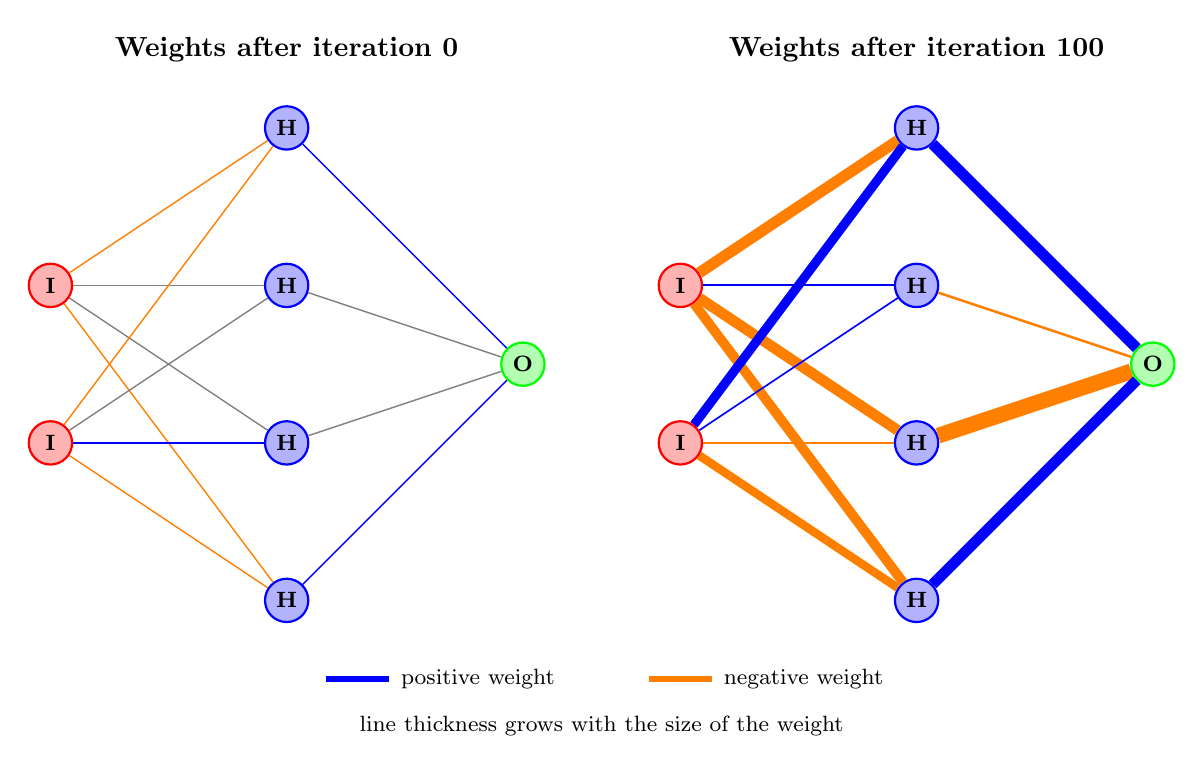
\begin{tikzpicture}[font=\small,
    inp/.style={circle, draw=red, thick, fill=red, fill opacity=0.3, text opacity=1, font=\footnotesize\bfseries, minimum size=0.55cm, inner sep=0pt},
    hid/.style={circle, draw=blue, thick, fill=blue, fill opacity=0.3, text opacity=1, font=\footnotesize\bfseries, minimum size=0.55cm, inner sep=0pt},
    outp/.style={circle, draw=green, thick, fill=green, fill opacity=0.3, text opacity=1, font=\footnotesize\bfseries, minimum size=0.55cm, inner sep=0pt}]
  \begin{scope}[xshift=0cm]
    \node[font=\bfseries] at (3,7.0) {Weights after iteration 0};
    \node[inp] (I1) at (0,4) {I};
    \node[inp] (I2) at (0,2) {I};
    \node[hid] (H1) at (3,6) {H};
    \node[hid] (H2) at (3,4) {H};
    \node[hid] (H3) at (3,2) {H};
    \node[hid] (H4) at (3,0) {H};
    \node[outp] (O) at (6,3) {O};
    \draw[orange, line width=0.52pt] (I1) -- (H1);
    \draw[gray, line width=0.50pt] (I1) -- (H2);
    \draw[gray, line width=0.50pt] (I1) -- (H3);
    \draw[orange, line width=0.51pt] (I1) -- (H4);
    \draw[orange, line width=0.51pt] (I2) -- (H1);
    \draw[gray, line width=0.50pt] (I2) -- (H2);
    \draw[blue, line width=0.52pt] (I2) -- (H3);
    \draw[orange, line width=0.51pt] (I2) -- (H4);
    \draw[blue, line width=0.52pt] (H1) -- (O);
    \draw[gray, line width=0.50pt] (H2) -- (O);
    \draw[gray, line width=0.50pt] (H3) -- (O);
    \draw[blue, line width=0.51pt] (H4) -- (O);
  \end{scope}
  \begin{scope}[xshift=8cm]
    \node[font=\bfseries] at (3,7.0) {Weights after iteration 100};
    \node[inp] (I1) at (0,4) {I};
    \node[inp] (I2) at (0,2) {I};
    \node[hid] (H1) at (3,6) {H};
    \node[hid] (H2) at (3,4) {H};
    \node[hid] (H3) at (3,2) {H};
    \node[hid] (H4) at (3,0) {H};
    \node[outp] (O) at (6,3) {O};
    \draw[orange, line width=4.04pt] (I1) -- (H1);
    \draw[blue, line width=0.67pt] (I1) -- (H2);
    \draw[orange, line width=3.90pt] (I1) -- (H3);
    \draw[orange, line width=3.53pt] (I1) -- (H4);
    \draw[blue, line width=3.30pt] (I2) -- (H1);
    \draw[blue, line width=0.59pt] (I2) -- (H2);
    \draw[orange, line width=0.54pt] (I2) -- (H3);
    \draw[orange, line width=3.08pt] (I2) -- (H4);
    \draw[blue, line width=3.94pt] (H1) -- (O);
    \draw[orange, line width=0.91pt] (H2) -- (O);
    \draw[orange, line width=5.67pt] (H3) -- (O);
    \draw[blue, line width=3.89pt] (H4) -- (O);
  \end{scope}
  \draw[blue, line width=2pt] (3.5,-1.0) -- (4.3,-1.0) node[right, black, font=\footnotesize] {positive weight};
  \draw[orange, line width=2pt] (7.6,-1.0) -- (8.4,-1.0) node[right, black, font=\footnotesize] {negative weight};
  \node[font=\footnotesize] at (7,-1.6) {line thickness grows with the size of the weight};
\end{tikzpicture}
